% !TEX root = ../thesis.tex
\section{Cross-System Communication Using Queries}\label{sec:comm}

The Math-In-The-Middle approach and the implementation including virtual theories has been discussed. 
QMT, a query language for \mmt\ has also been described. 
This section focuses on how to make use of these concepts to enable transparent system interaction. 

So far, QMT has only been used on concrete \mmt\ content, and in particular the evaluation has made use of indexes. 
These indexes are built incrementally -- each time new content is added to \mmt, it is added to the index. 
Content can only be found using QMT if it is stored in the index. 

\subsection{Avoiding Reliance on In-Memory Content}\label{sec:comm:reliance}

Recall that virtual theories only load content lazily -- exactly when it is required. 
This means that an item is only added to the index -- and can only be found by QMT queries -- once it is explicitly requested by the user. 
Thus if the user wants to properly resolve a query, they first have to load all potential results into \mmt memory. 
This is best illustrated with an example. 

\begin{example}\label{example:lmfdbhard}
	The query \begin{lstlisting}[language=qmt]
Related(
	URI('lmfdb:db/transitivegroups?groups'),
	ToObject(Declares())
)
	\end{lstlisting} when evaluated should return the URI of all known transitive groups.
\end{example}

To evaluate this query, the existing implementation would first look into the index for binary predicates to find all URIs that are related to the transitive group theory by the given \inlinecode{Declares()} relation.
Here is where the problem comes in -- where does this index come from?

In order to build such an index, (at the very least) a complete list of available groups is required.
By nature of being a virtual theory, such a list never exists in \mmt\ memory by default -- since the backend for the transitive groups theory only loads the set of declarations that is needed.
Thus such an index is at most partial -- and may not exist at all.

The same not only goes for this specific QMT query -- it holds for all queries sent to virtual theories. 
As seen, evaluation can break easily and may only return partial results, if any at all. 
This limitation makes search fairly useless for virtual theories. 
Furthermore, it also negates the advantage of virtual theories. 
These were built so that not all content has to be loaded from an external system into memory. 


Thus the evaluation of queries had to be reworked. 
There are several approaches to achieve this. 

One obvious approach involves loading all relational information into memory.
Once this is available, the same strategies as for concrete theories can be used. 
This still poses a similar problem to the one that virtual theories are trying to solve in the first place. 
Such an approach still needs to load information about the entire external database into the \mmt\ system -- albeit to a lesser degree because only need the relational information.
Thus this solution is not a desirable one. 

\subsection{Making Use of Existing Querying Mechanisms}\label{sec:comm:existing}

Most external systems already have some form of information retrieval mechanism -- commonly in the form of a query language or an API. 
And indeed, in the case of \lmfdb, such an API exists.

One can send queries to the underlying MongoDB implementation.
Answering Example~\ref{example:lmfdbhard} seems almost trivial -- a simple \inlinecode{GET} request to \url{http://www.lmfdb.org/api/transitivegroups/groups/?_offset=0&_format=json} is enough.
The \lmfdb\ API is also capable of answering more interesting queries. 

This provides a new approach for making queries towards virtual theories. 
First, the \mmt\ query is translated into a system-specific information-retrieval language -- in the case of \lmfdb\ this is a MongoDB-based syntax.
Next, this translated query is sent to the external API. 
Upon receiving the results, these are translated back into \omdocmmt\ with the help of already existing functionality in the appropriate virtual theory backend.

This leaves just one problem unsolved -- translating queries into the system-specific API. 
Consider that it is not sufficient to just translate all queries. 
One hand a general QMT query may or may not involve a virtual theory. 
On the other hand, it may also involve several unrelated virtual theories. 
This makes it necessary to filter out queries involving virtual theories, so that they can be evaluated properly. 

Achieving this automatically is a non-trivial problem. 
Queries are inductive in nature, along with their evaluation. 
In principle, one could intercept each of the intermediate results. 
However, this would require a check on each intermediate result to determine if it comes from a virtual theory or not, 

Recall that queries may return URIs, Objects and String literals. 
Inspecting URIs is rather simple, but this is not the case for objects. 
The objects themselves are inductive in structure and thus recursing through the entire structure would become necessary. 

Thus such an approach would be very expensive computation wise and would not scale if a query returns a large set of objects. 
This would not only cause a performance hit, but also make for a much more complicated codebase. 
After each intermediate result one potentially has to switch the entire evaluation strategy.

\subsection{Annotating Sub-Queries for External Systems}\label{sec:comm:iop}

Instead, during this project a new type of query was introduced -- the \inlinecode{I($\meta{query}$, $\meta{hint}$)} operator.
The first parameter of this is a query that is to be evaluated, and the second one is a so-called evaluation hint that describes how the query should be evaluated.
This second parameter currently is a simple string. 

The goal of this type of query is to annotate a sub-query and tell the implementation to use a specific external theory to evaluate it. 
Each virtual theory backend can register a \identifier{QueryEvaluationExtension}. 
This is responsible for translating these sub-queries and retrieving the appropriate results. 

With this new operator, Example~\ref{example:lmfdbhard} becomes:

\begin{example}\label{example:lmfdbhint}
  Example~\ref{example:lmfdbhard} annotated with the \inlinecode{I()} operator. 
	\begin{lstlisting}[language=qmt]
I(
	Related(
		URI('lmfdb:db/transitivegroups?groups'),
		ToObject(Declares())
	), 
	'lmfdb'
)
	\end{lstlisting}
\end{example}

Evaluation of such a query is straightforward. 
If this query is encountered during query evaluation, the implementation finds the \inlinecode{QueryEvaluationExtension} identified by the hint. 
Then it turns over control to the extension and allows it to evaluate results. 
Once the results are available, control is passed back to the normal QMT evaluator which continues evaluating as normal. 
Here, this query is used for virtual theories, however it could in principal be used to implement other evaluation strategies as well. 

This procedure has turned out to work very well in practice. 
However, this does not fully address our requirement. 
The user needs to explicitly mark up virtual theories and thus they are not as transparent as originally desired. 

\subsection{Calling the LMFDB API}\label{sec:comm:lmfdbapi}

It is not easily possible to translate all queries into \lmfdb\ Queries. 
The purpose of this subsection is to give the reader an insight into which queries can be translated and how this is achieved. 

To identify this subset of translatable queries, we look into the structure of knowledge stored in \lmfdb. 
Recall from Section~\ref{sec:vt:lmfdb} that each item is essentially a set of key-value pairs. 
As such, interesting queries usually take the form of ``find all objects in this \lmfdb\ database where some specific key equals a specific value''. 

\begin{example}\label{example:lmfdblong}
	The query
	\begin{lstlisting}[language=qmt]
I(
	Comprehension(
		Related(
			URI('lmfdb:db/transitivegroups?group'), 
			ToObject(Declares())
		), 
		LocalName('x'), 
		Holds(
			Bound(x), 
			Equals(
				'x', 
				OMV(LocalName('x')), 
				OMA(
					OMID('mitm:smglom/algebra?magma?commutative'), 
					OMV(LocalName('x'))
				), 
				OMLIT(mitm:Foundation?Logic?bool?true)
			)
		)
	)
	, 'lmfdb'
)
\end{lstlisting} finds all commutative transitive groups known to \lmfdb. 
\end{example}

This example is typical for queries that can be translated into \lmfdb. 
It begins on the outside with the \identifier{I} operator, to indicate that this is a query to be evaluated using \lmfdb. 
Next comes a composite query built using the \identifier{Comprehension} operator. 
This operator is applied to two main arguments, (1) the set of all transitive groups (recall example~\ref{example:lmfdbhard} above) and (2) a predicate that checks if a group is commutative. 

To translate this QMT query into an \lmfdb\ query, two main steps need to be performed. 
First, the sub-database of \lmfdb\ that is involved needs to be found. 
This can be determined from the first argument to the Comprehension operator, here this is the \identifier{transitivegroups} database. 
Second, the groups to select from the database need to be selected. 

This second step is the more restrictive one.
We need to have a closer look at the \identifier{Equals} judgment \begin{lstlisting}[language=qmt]
Equals(
	'x', 
	OMV(LocalName('x')), 
	OMA(
		OMID('mitm:smglom/algebra?magma?commutative'), 
		OMV(LocalName('x'))
	), 
	OMLIT(mitm:Foundation?Logic?bool?true)
)
\end{lstlisting}. 

This again has several arguments, \begin{itemize}
	\item a left hand side and a right hand side of the equality to be checked and 
	\item a variable (here $x$) that needs to be substituted.
\end{itemize}
The left hand side of the equality is given by the application of \uri{mitm:smglom/algebra?magma?commutative} onto this variable. 
The right hand side is given by a literal value of true. 
Thus it can be inferred that \lmfdb\ should return all groups for which the key corresponding to the \identifier{commutative} property has the literal value \inlinecode{true}. 

Next, one can make use of codecs to find the name of the field corresponding to the \identifier{commutative} property. 
This is the \identifier{ab} (as in abelian) field. 
Furthermore, the codecs can be used to translate the literal \inlinecode{true} into a JSON value understood by the \lmfdb\ API. 
Here, the codec \identifier{BooleanAsInt} is used and the value of \inlinecode{true} corresponds to $1$. 
This generates an API call to \url{http://www.lmfdb.org/api/transitivegroups/groups/?ab=i1&_offset=0&_format=json}. 

\subsection{QMT Queries as OpenMath Objects}\label{sec:comm:mmt}

Next, an introduction on how to send queries to \mmt is given. 
Previously, to send a query to \mmt, it was either required to directly interface with \mmt\ on a Scala level or to encode queries in an XML representation. 
The first approach is infeasible to most system as they can not access Scala objects natively. 
The second approach provides an \mmt\ specific XML syntax, that might not be easily adaptable by other systems. 

The SCSCP protocol described Section~\ref{sec:mitm:scscp} is designed to enable exactly the kind of interoperability that is needed here. 
It allows different mathematical knowledge systems to communicate using a common language, namely OpenMath objects. 
Thus it makes sense to represent queries as OpenMath objects, so that they can be communicated using this protocol. 

Recall that the QMT grammar is inductive. 
This enables representing each query as a term in \mmt. 

One can start by representing each terminal query and each query operator as an MMT symbol. 
Since the \identifier{Query} class recuses into \identifier{Prop}, \identifier{Unary}, \identifier{Binary}, \identifier{QueryJudgement} and other classes, it needs to be done for these as well. 
This gives a set of theories representing each class. 
These can be found in the namespace given by the \uri{qmt} abbreviation. 

This can be easily used to represent terminal queries, by using an appropriate reference to the symbol.
To represent a complex query, an application of the query operator symbol to the terms representing the query parameters. 
Furthermore, literals can be used for queries with integer and string parameters. 
Note that the \identifier{QueryJudgement} class recurses into the \identifier{Term} class which can be used directly -- no special symbols needed. 

Furthermore, special care needs to be taken of binding queries. 
Here a single application is not enough. 
As the name says, the queries are binding variables. 
Hence we can make use of a so-called binder term, an OpenMath term that allows the binding of variables. 

Recall that \mmt\ terms correspond to OpenMath objects. 
This means that if one can represent \identifier{Queries} as \mmt\ terms, one can also be represent them as OpenMath objects. 
In Examples~\ref{example:simpleOM} and \ref{example:lmfdblongOM} we can see the OpenMath objects\footnote{
  The syntax used in these examples is not valid OpenMath. 
  This would usually be represented using XML, however to make it easier on the reader an \mmt\ surface syntax like style is used. 
} that correspond to the Queries in
Examples~\ref{example:simple} and \ref{example:lmfdblong} respectively. 

\begin{example}\label{example:simpleOM}
  Example~\ref{example:simple} as an OpenMath object. 
  \begin{lstlisting}[language=qmt]
OMA(
  OMS(URI('qmt:?QMTQuery?Related')), 
  OMA(
    OMS(URI('qmt:?QMTQuery?Literal')), 
    OMS('odk:algebra?Semigroup')
  ),
  OMA(
    OMS(URI('qmt:?QMTRelationExp?ToObject')), 
    OMS(URI('qmt:?QMTBinaries?Declares'))
  )
)
  \end{lstlisting}
\end{example}

\begin{example}\label{example:lmfdblongOM}
	Example~\ref{example:lmfdblong} as an OpenMath object. 
	\begin{lstlisting}[language=qmt]
OMA(
  OMID(URI('qmt:?QMTQuery?I')), 
  OMBIND(
    OMID(URI('qmt:?QMTQuery?Comprehension'))
    OMV(LocalName('x')), 
    OMA(
      OMS(URI('qmt:?QMTQuery?Related')), 
      OMA(
        OMS(URI('qmt:?QMTQuery?Literal')), 
        OMS('lmfdb:db/transitivegroups?group')
      ),
      OMA(
        OMS(URI('qmt:?QMTRelationExp?ToObject')), 
        OMS(URI('qmt:?QMTBinaries?Declares'))
      )
    ),
    OMA(
      OMID('Holds')
      OMV(LocalName('x')),
      OMBIND(
        OMID(URI('qmt:?QMTJudgements?Equals'))
        OMV(LocalName('x')), 
        OMA(
          OMID('mitm:smglom/algebra?magma?commutative'), 
          OMV(LocalName('x'))
        ), 
        OMLIT(mitm:Foundation?Logic?bool?true)
      )
    )
  ), 
  OMSTR('lmfdb')
)
\end{lstlisting}
\end{example}

\subsection{Using MMT Surface Syntax}\label{sec:omqueries:surface}

The above examples demonstrate that the OpenMath syntax of queries almost directly corresponds to the inductive structure of QMT. 
This OpenMath approach easily allows computer systems to formulate queries, however it is equally complex to create queries in for a human. 
To make \mmt\ queries accessible for humans, it is necessary to design a more human-readable syntax. 

Recall that \mmt\ terms can be parsed from the human-writable \mmt\ surface syntax. 
With the help of notations,  syntax for queries that can be both read and written by end-users can be defined. 
When designing such a syntax to be parsed by \mmt, two factors need to be taken into account. 

First, each query usually contains a multitude of query operators and references to content within \mmt. 
This poses a problem because both need to refer the symbols representing the query operators and the actual symbols somewhere inside of \mmt\ as symbols. 

\begin{example}\label{example:simpleSurface}
  Example~\ref{example:simple} as an \mmt\ object in surface syntax.  
  \begin{lstlisting}[language=qmt]
related to ( literal `odk:algebra?Semigroup ) by (object declares)
  \end{lstlisting}
\end{example}

An example makes this problem more obvious. 
Consider Example~\ref{example:simpleSurface}, specifically the inner part \inlinecode{ literal `odk:algebra?Semigroup } only. 
This corresponds to a \identifier{Literal} query with an argument of \uri{odk:algebra?Semigroup}. 
One needs to make sure that the second argument to this query is parsed as a literal of a given URL, and not as part of the query syntax. 
To achieve this, one uses a generic feature in the \mmt\ parser and simply mark it as a literal by prefixing it with \inlinecode{`}. 

\begin{example}\label{example:lmfdblongSurface}
  Example~\ref{example:lmfdblong} as an \mmt\ object in surface syntax.  
  \begin{lstlisting}[language=qmt]
use "lmfdb" for {*
  x in (
    related to ( literal `lmfdb:db/transitivegroups?group ) by (object declares)
  ) | holds x (
    x commutative x *=* true
  )
*}
\end{lstlisting}
\end{example}

The second and related problem comes when using \mmt\ terms within parts of a query. 
Consider Example~\ref{example:lmfdblongSurface}. 
Here, inside the \identifier{holds} part of the query, one wants to find all groups inside of \lmfdb\ that are commuatative. 
This is written as \inlinecode{commutative x *=* true}. 
Here it is not that difficult to separate the actual terms from the query level, but in a general scenario, there could be an arbitrary term instead. 
This could contain any kind of references to any kind of symbols inside of \mmt. 

To solve this problem, one has to make sure to always find all query level operators first, then construct an \mmt\ term representing the query and finally parse the internal \mmt\ terms. 
This is achieved by giving the Query operators a lower precedence in parsing. 
Furthermore, to make sure that all sub-terms are parsed correctly, one makes sure that \mmt\ knows the theory these literal terms come from, by adding an appropriate reference to the context the entire syntax is parsed in.  

\subsection{Sending Queries from the Web}\label{sec:comm:web}

We discuss how to make use of the QMT query language. 
We have looked at QMT and seen how it can be used to enable transparent cross-system communication and distributed computation. 
Furthermore, we have seen how it can be given both a human readable and machine readable syntax. 

The next step is to expose an interface for queries to be sent to the \mmt\ system and be evaluated.

The first thing we want to do is build an API with which other systems can send QMT Queries to \mmt\ and receive responses. 
A common way for almost any kind of software systems to communicate is via an HTTP based API - a RESTful interface. 
This is easy to implement in almost any kind of programming language and thus enables a broad set of clients to communicate with \mmt\ efficiently. 

\mmt\ already has a built-in webserver and also an extension mechanism that allows plugins to add custom functionality to it. 
Prior to this project, a minimal plugin that allowed to send queries in a legacy XML-based syntax existed. 
This plugin has been refactored and extended to support surface syntax, as shown in Section~\ref{sec:omqueries:surface}. 

Upon receiving a query from a client, this plugin first parses the syntax and converts it into the internal data structure representing the query, before type checking it to ensure validity. 
Next, the plugin evaluates the query using the procedures described in Sections~\ref{sec:qmt:eval} and \ref{sec:comm:lmfdbapi}.
Finally, the result is serialized into XML and sent back to the client. 


To demonstrate this interface and make it accessible to users a web interface has also been implemented. 
Screenshots of the interface can be found in Figures~\ref{fig:webinterface:entering} and \ref{fig:webinterface:results}. 

% !TEX root = ../thesis.tex
\begin{figure}[h]
  \begin{center}
    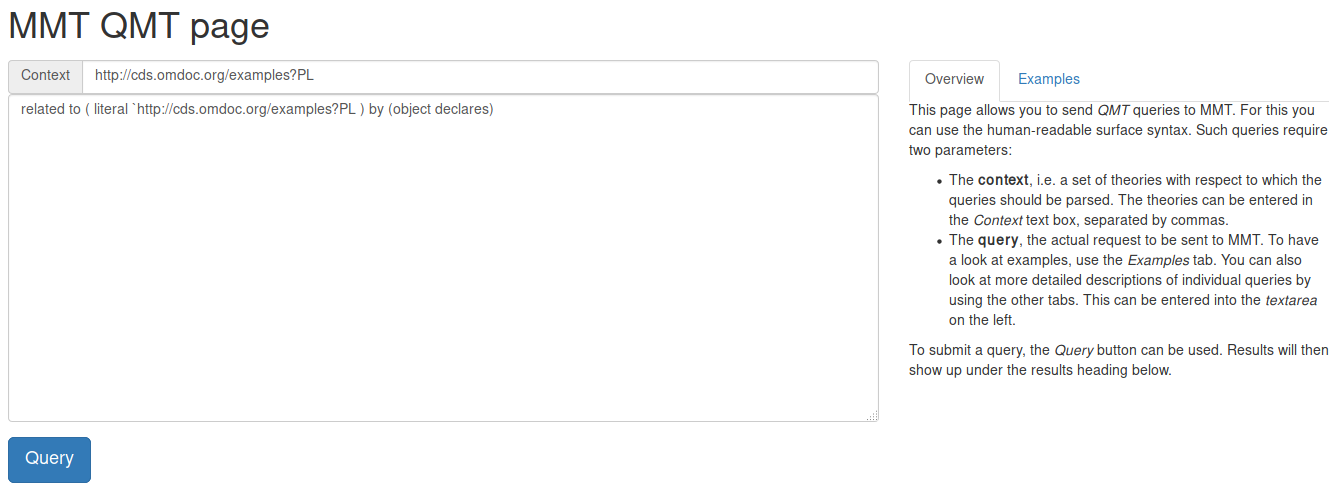
\includegraphics[width=1.0\textwidth]{imgs/QMTquery.png}
  \end{center}
  \caption{QMT Web Interface for entering Queries. }
  \label{fig:webinterface:entering}
\end{figure}

\begin{figure}[h]
  \begin{center}
    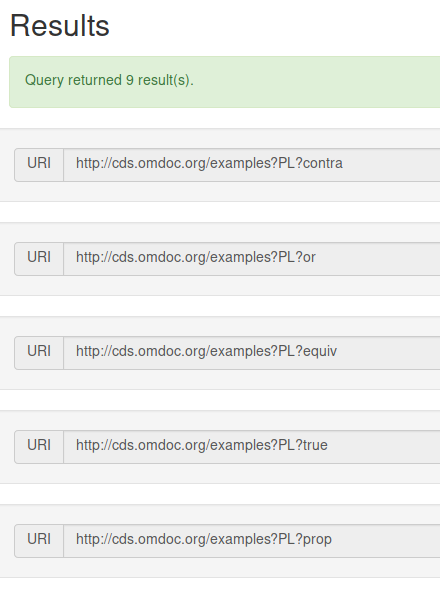
\includegraphics[width=0.5\textwidth]{imgs/QMTresults.png}
  \end{center}
  \caption{QMT Web Interface for displaying results. }
  \label{fig:webinterface:results}
\end{figure}

The web interface consists of two parts, an interface to enter queries as well as a result listing. 

The interface for entering queries can be seen in Figure~\ref{fig:webinterface:entering}. 
To submit a query, the user has to fill out two fields and click the \identifier{Query} button. 
The fields to be filled are the context and the query itself. 

As described previously, the context is a set of theories with respect to which the queries should be parsed. 
It can be entered in the \identifier{Context} text box separated by commas. 
The query, in surface syntax, can be entered in the main text area on the left. 

The display of results can be found in Figure~\ref{fig:webinterface:results}. 
On the web interface this is located below the entering interface and only shows up once results have been received. 
The interface is very plain and only shows two pieces of information, the number of results and each individual result. 